Thinking...
The user asks: translate the Japanese sentence to English, but there is TeX code inserted, which should be output unchanged. The Japanese text: "以下のの日本語文を英訳してください。ただしTeXのコードが挿入されているのでその部分はそのまま出力してください：" then the TeX figure environment is shown. So we need to translate the Japanese description? Actually the request: "以下のの日本語文を英訳してください。ただしTeXのコードが挿入されているのでその部分はそのまま出力してください：" then the code block containing the figure environment. So we need to produce the English translation of the Japanese text within the figure caption perhaps? The figure includes caption in Japanese: "新規出現高被引用論文の高被引用論文に占める割合（\%）". So translate that caption to English, but keep the rest unchanged. So output should be same TeX code but caption translated. Keep all other TeX code unchanged.

Thus output:

\begin{figure}[h]
\begin{center}
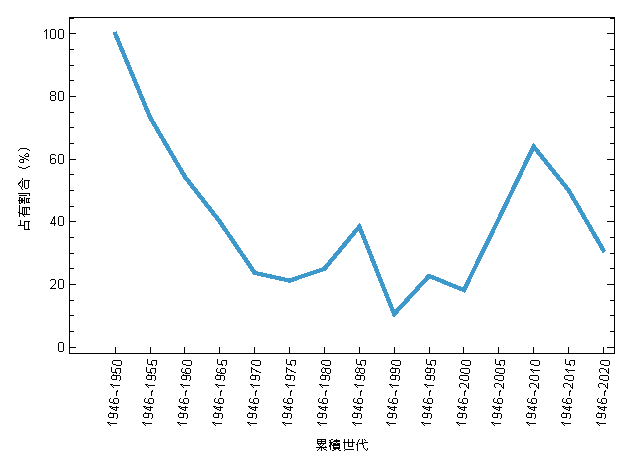
\includegraphics[width=76mm]{gr5.eps}
\caption{Proportion (\%) of newly emerging highly cited papers among highly cited papers}
\label{fig:gr5}
\end{center}
\end{figure}

Check translation: "新規出現高被引用論文の高被引用論文に占める割合（\%）" literally: "The percentage (%) of newly emerging highly cited papers that constitute highly cited papers". Better: "Percentage of newly emerging highly cited papers among highly cited papers (%)". That is fine.

Thus produce final answer with code unchanged except caption.
...done thinking.

\begin{figure}[h]
\begin{center}
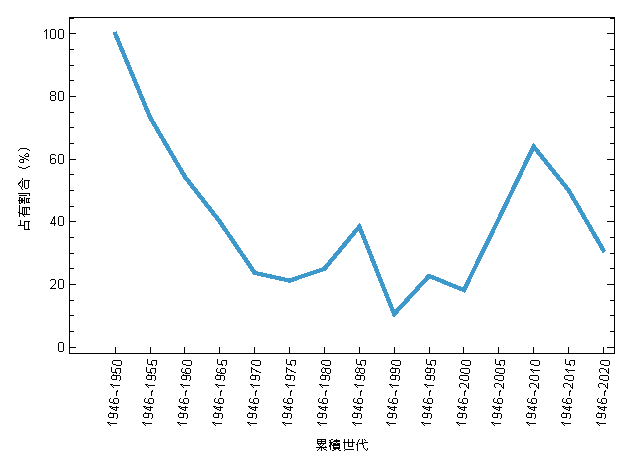
\includegraphics[width=76mm]{gr5.eps}
\caption{Percentage (\%) of newly emerging highly cited papers among highly cited papers}
\label{fig:gr5}
\end{center}
\end{figure}

